
\title{A Comparison of Dimensionality Reduction Techniques for Robotic Motion
Planning}

\date{\today}

\author{Brandon Araki \and Alex Wallar}

\documentclass[12pt]{article}

\usepackage[pdftex]{graphicx}
\graphicspath{{figs/}}
\usepackage{subcaption}

\usepackage{amsmath}
\usepackage{amssymb}
\usepackage{mathabx}

\usepackage{mathptmx}
\DeclareMathAlphabet{\mathcal}{OMS}{cmsy}{m}{n}

\usepackage{relsize}

\usepackage{float}

\usepackage{algorithm}

\usepackage[noend]{algorithmic}

\floatstyle{ruled} \newfloat{program}{thp}{lop} \floatname{program}{Structure}

\newcommand{\Normal}[3]{\mathcal{N}(#1, #2, #3)}

\newcommand{\Acronym}[1]{\ensuremath{{\small{\texttt{#1}}}}}
\newcommand{\Name}{\Acronym{Camgaze.js}} \newcommand{\False}{\Constant{false}}
\newcommand{\True}{\Constant{true}}
\newcommand{\Symbol}[1]{\ensuremath{\mathcal{#1}}}
\newcommand{\Function}[1]{\ensuremath{{\small \textsc{#1}}}}
\newcommand{\Constant}[1]{\ensuremath{\small{\texttt{#1}}}}
\newcommand{\Var}[1]{\ensuremath{{\small{\textsl{#1}}}}}
\newcommand{\argmin}[1]{\underset{#1}{\operatorname{arg}\,\operatorname{min}}\;}
\newcommand{\grad}[1]{\underset{#1}{\operatorname{\Function{GradientDecent}}}\;}

\newcommand{\xr}[0]{\ensuremath{{x_{\Var{rand}}}}}
\newcommand{\xnear}[0]{\ensuremath{{x_{\Var{near}}}}}
\newcommand{\xnearest}[0]{\ensuremath{{x_{\Var{nearest}}}}}
\newcommand{\xnew}[0]{\ensuremath{{x_{\Var{new}}}}}
\newcommand{\xmin}[0]{\ensuremath{{x_{\Var{min}}}}}
\newcommand{\xparent}[0]{\ensuremath{{x_{\Var{parent}}}}}
\newcommand{\cmin}[0]{\ensuremath{{c_{\Var{min}}}}}
\newcommand{\cost}[0]{\ensuremath{{\Function{Cost}}}}
\newcommand{\linef}[1]{\ensuremath{{c(\Function{Line}(#1))}}}

\begin{document}

\maketitle

\section{Background}

Dimensionality reduction is a key component of making robotic motion planning
fast and efficient. A rigid body has six degrees of freedom (DoF), so a
multi-link robot such as a humanoid or snake robot can have dozens or hundreds
of DoF. The rotational and translational transformations of a rigid body can be
described with the 3-dimensional Special Euclidean group (known as SE(3)).
SE(3) is homeomorphic to the topological space
$\mathbb{R}^3\bigtimes\mathbb{RP}^3$ (where $\mathbb{RP}^3$ is the
3-dimensional real projective plane). Therefore it is easy to imagine a
multi-link robot \cite{kuindersma2015optimization} or a multi-robot system
\cite{alonso2015multi} with an arbitrarily complex state space. The picture is
further complicated by the addition of obstacles into a robot's world. The
state space for motion planning, which must take into account both the robot
and obstacles, is called the configuration space (or C-space)
\cite{lozano1983spatial}. 

Motion planning essentially consists of a search over the configuration space
from a start configuration to a goal configuration. A huge number of methods
for searching through the configuration space have been developed, most of
which can be divided into two classes, sampling-based motion planning and
combinatorial motion planning \cite{lavalle2006planning}. In sampling-based
motion planning, obstacles in the C-space are defined implicitly so that the
path is constructed by randomly or pseudorandomly sampling points from the
C-space, doing collision checking, and connecting valid points to their nearest
neighbors. In combinatorial motion planning, obstacles are defined explicitly
and a complete search of the C-space is made. Because of the difficulty of
explicitly defining all of the geometry in a potentially complex world,
sampling-based motion planning techniques such as the Rapidly expanding Random
Tree (RRT) and the Probabilistic RoadMap (PRM) are the most popular motion
planning techniques.

We used PRM and RRTConnect in our project. 

\subsection{PRM}

The Probabilistic RoadMap algorithm has two phases: the preprocessing phase in
which a roadmap is constructed by sampling random points in the C-space, and
the query phase in which a graph search over the roadmap is made to connect
initial and goal configurations \cite{kavraki1996prm}. The map is constructed
during the preprocessing phase by sampling random points in the C-space and
then adding them to the vertices in the roadmap within a certain radius of the
point. The algorithm is described in Alg~\ref{alg:PRM}.
%PRM can be elevated to the asymptotically optimal PRM*, which is
%described in Alg~\ref{alg:PRMstar}, by defining the radius to be a function of
%the number of vertices and the dimensionality of the space
%\cite{karaman2011sampling}. Since PRM* is asymptotically optimal, its solution
%will converge to the optimal path as time goes to infinity.

\subsection{RRTConnect}

The Rapidly exploring Random Tree algorithm works by building up a tree from
the initial configuration to the goal configuration \cite{lavalle1998rrt}.
Starting with the initial configuration as the root, it incrementally attempts
to add randomly selected samples to the tree until it reaches the goal
configuration.  The tree is ``rapidly exploring'' because the sample selection
is biased towards areas with large Voronoi regions (where the Voronoi regions
are computed based off of the nodes of the tree). RRTConnect, which is
described in Algos.~\ref{alg:extend_RRT},~\ref{alg:connect_RRT},
and~\ref{alg:RRTConnect}, differs from RRT in that two trees, one with its root
at the initial configuration and one with its root at the start configuration,
grow towards each other \cite{kuffner2000rrt}.
%RRT*, which is described in Alg~\ref{alg:RRTstar} differs from RRT in that for every new node, connections are tested to the new node from every other node that is within a certain radius from the new node \cite{karaman2011sampling}. The the tree is pruned so that edges that are not part of the shortest path from the root of the tree to the new node are removed. 

\section{Problem Description}

Despite the efficiency of sampling-based search, the high dimensionality of the
configuration space of complex robots means that motion planning for many
robots is slow or infeasible. This is because of the ``curse of dimensionality",
in which the size of the search space increases exponentially with the
dimension. One way to speed up motion planning is to reduce the dimensionality
of the C-space and do search in this reduced dimensionality space. For this
project, we tested the performance of a number of dimensionality reduction
techniques to see which one was the most effective in speeding up motion
planning while providing reliable obstacle avoidance.

\section{Dimensionality Reduction}

We used Feature Agglomeration, Truncated SVD, PCA, and Randomized PCA to
perform dimensionality reduction. We will briefly summarize each of these
techniques.

\subsection{PCA}

Principle Component Analysis, or PCA, transforms a set of variables into their
``principal components", or linearly uncorrelated variables
\cite{shlens2014pca}. Given an $m \times n$ matrix $\mathbf{X}$, you can find
its principal components by finding an orthonormal matrix $\mathbf{P}$ in $
\mathbf{Y} = \mathbf{PX} $ such that $\mathbf{C_Y} = \mathbf{YY}^T/n$. The rows
of $\mathbf{P}$ are the principal components of $\mathbf{X}$. In other words,
the axes of the dataset in question are reoriented so that the covariance of
the data along the first axis is minimized. After the first axis has been set,
the second axis is then set to minimize the covariance of the dataset along
that axis, and so on, so that the first axis has the lowest covariance, the
second axis has the second lowest, and so on. Dimensionality reduction is then
performed by chopping off the axes with the high covariance.

\subsection{Randomized PCA}

In Randomized PCA, computations are sped up by only approximating the singular
vectors of the components.

\subsection{Feature Agglomeration}

Feature Agglomeration is a form of hierarchical clustering in which clusters
are merged or split successively \cite{featureagglomeration}. Feature
Agglomeration groups together similar features to reduce the number of
features. It does this by using agglomerative clustering, in which every data
point starts as a cluster, and clusters are merged together.

\subsection{Truncated SVD}

In singular value decomposition, a matrix $\mathbf{M}$ is factorized into the
form $\mathbf{U} \Sigma \mathbf{V^*}$. $\Sigma$ is a diagonal matrix, and the
entries of $\Sigma$ are the singular values of $\mathbf{M}$. In Truncated SVD,
$\mathbf{M}$ is approximated by matrices $\mathbf{U_k} \Sigma_k
\mathbf{V^*_k}$, where $ k < r $, $r$ being the number of non-zero singular
values of the matrix \cite{maciejewski1989svd}. In effect you are approximating
$\mathbf{M}$ by cutting off low-value singular values. In this sense Truncated
SVD is similar to PCA; however, instead of cutting off the lowest eigenvalues
of the coviarance matrix, you are cutting off the singular values of the
matrix.

\section{Methods}

\subsection{Simplifications}

Although our aim is to show how dimensionality reduction techniques can speed
up motion planning for robots, doing motion planning for an actual robot is
very hard (specifying link geometry, defining constraints between links, etc).
Therefore we limited ourselves to path planning for a point in $\mathbb{R}^n$,
and we approximated obstacles as being convex polytopes. This is a valid
simplification of the robot motion planning problem for several reasons. The
first reason is that most real robots actually operate in a C-space similar to
$\mathbb{R}^n$. This is because $\mathbb{RP}^3$, the space in which the
rotation of a rigid body occurs, simplifies to $\mathbb{R}^3$ if the joint
cannot make a full rotation. Second, in defining the C-space, the obstacle
space takes into account the interaction of the robot geometry with obstacles.
Therefore motion planning through the free space can be done using a point to
represent the robot (since the geometry of the robot is implicitly included in
the obstacle space). Therefore, although our simulations do not represent real
robots and real obstacles, they do approximate them.

\subsection{Experimental Setup}

We implemented an n-dimensional world in which to test these algorithms. We
structured our code so that we could run our tests in any space of dimension $d
\geq 2$. We also made visualization scripts for the 2 and 3 dimensional tests.
Examples of randomly generated 2D and 3D scenes with candidate solution paths
can be seen in Fig.~\ref{fig:examples}.

Next we made a random obstacle generator. We create n-dimensional convex
polytopes by sampling $n^{2}$ random points within the $n$-sphere. To generate
a single point, you must sample $n - 1$ angles from a uniform distribution
between 0 and $2\pi$, $n$ radii from a Gaussian distribution,
$\mathcal{N}(r_{\mu}, r_{\sigma})$ where $r_{\mu}$ and $r_{\sigma}$ are the
mean and standard deviation for the radius of the convex polytope, and $n$
floats to act as the center of the $n$-sphere.  Then you use the series of
equations in Eq.~\ref{eq:nsphere} to produce a randomly sampled point within
the $n$-sphere where $c_k$, $r_k$, and $\phi_k$ are the centers, radii, and
angles respectively.  To produce a convex polytope, we then computed the
$n$-dimensional convex hull over these points. The convex hull then provided
the normal equations and offsets for each facet on the polytope.

\begin{align}
    \begin{split}
        x_1 &= c_1 + r_1 \cos(\phi_1) \\
        x_2 &= c_2 + r_2 \sin(\phi_1) \cos(\phi_2) \\
        x_3 &= c_3 + r_3 \sin(\phi_1) \sin(\phi_2) \cos(\phi_3) \\
            &\vdots\\
        x_{n-1} &= c_{n - 1} + r_{n - 1} \sin(\phi_1) \cdots \sin(\phi_{n-2}) \cos(\phi_{n-1}) \\
        x_n &= c_n + r_{n} \sin(\phi_1) \cdots \sin(\phi_{n-2}) \sin(\phi_{n-1}) \,.
    \end{split}
    \label{eq:nsphere}
\end{align}

After generating random obstacles, we ran Feature Agglomeration, Truncated SVD,
PCA, and Randomized PCA to reduce the dimensionality of the space by using the
sampled points within each $n$-sphere as training data. We then ran PRM* and
RRTConnect on each of these reduced dimensionality spaces, as well as on the
fully-dimensional space as a control. We then ran an inverse transform on the
paths that we find to return them to the fully-dimensional space in order to
verify that the path in the reduced dimension did not come into collision with
obstacles. We collected data on the number of runs that fail to find a
solution, the time it takes to run the algorithm, and the length of the
solution if one was found.  A summary of this paragraph can be found in
Algo.~\ref{alg:DR}.

For our experiments, we varied the number of random obstacles in the scene, the
planning algorithm used, and the method of dimensionality reduction. For each
problem instance, the random generator was seeded in order to make fair
comparisons between the planners and dimensionality reduction techniques.
Also, since the algorithms are non-deterministic, each problem instance
executed 100 times. We used scenes with 250, 300, and 350 obstacles in order to
measure how the planners and dimensionality reduction techniques vary in their
performance with varying levels of obstacle density. In the results presented,
we are reducing from 8 dimensions to 6 dimensions and using mean radius of
$14.8$ for the convex polytopes.

\section{Results}

\begin{figure}[h!]
    \centering
    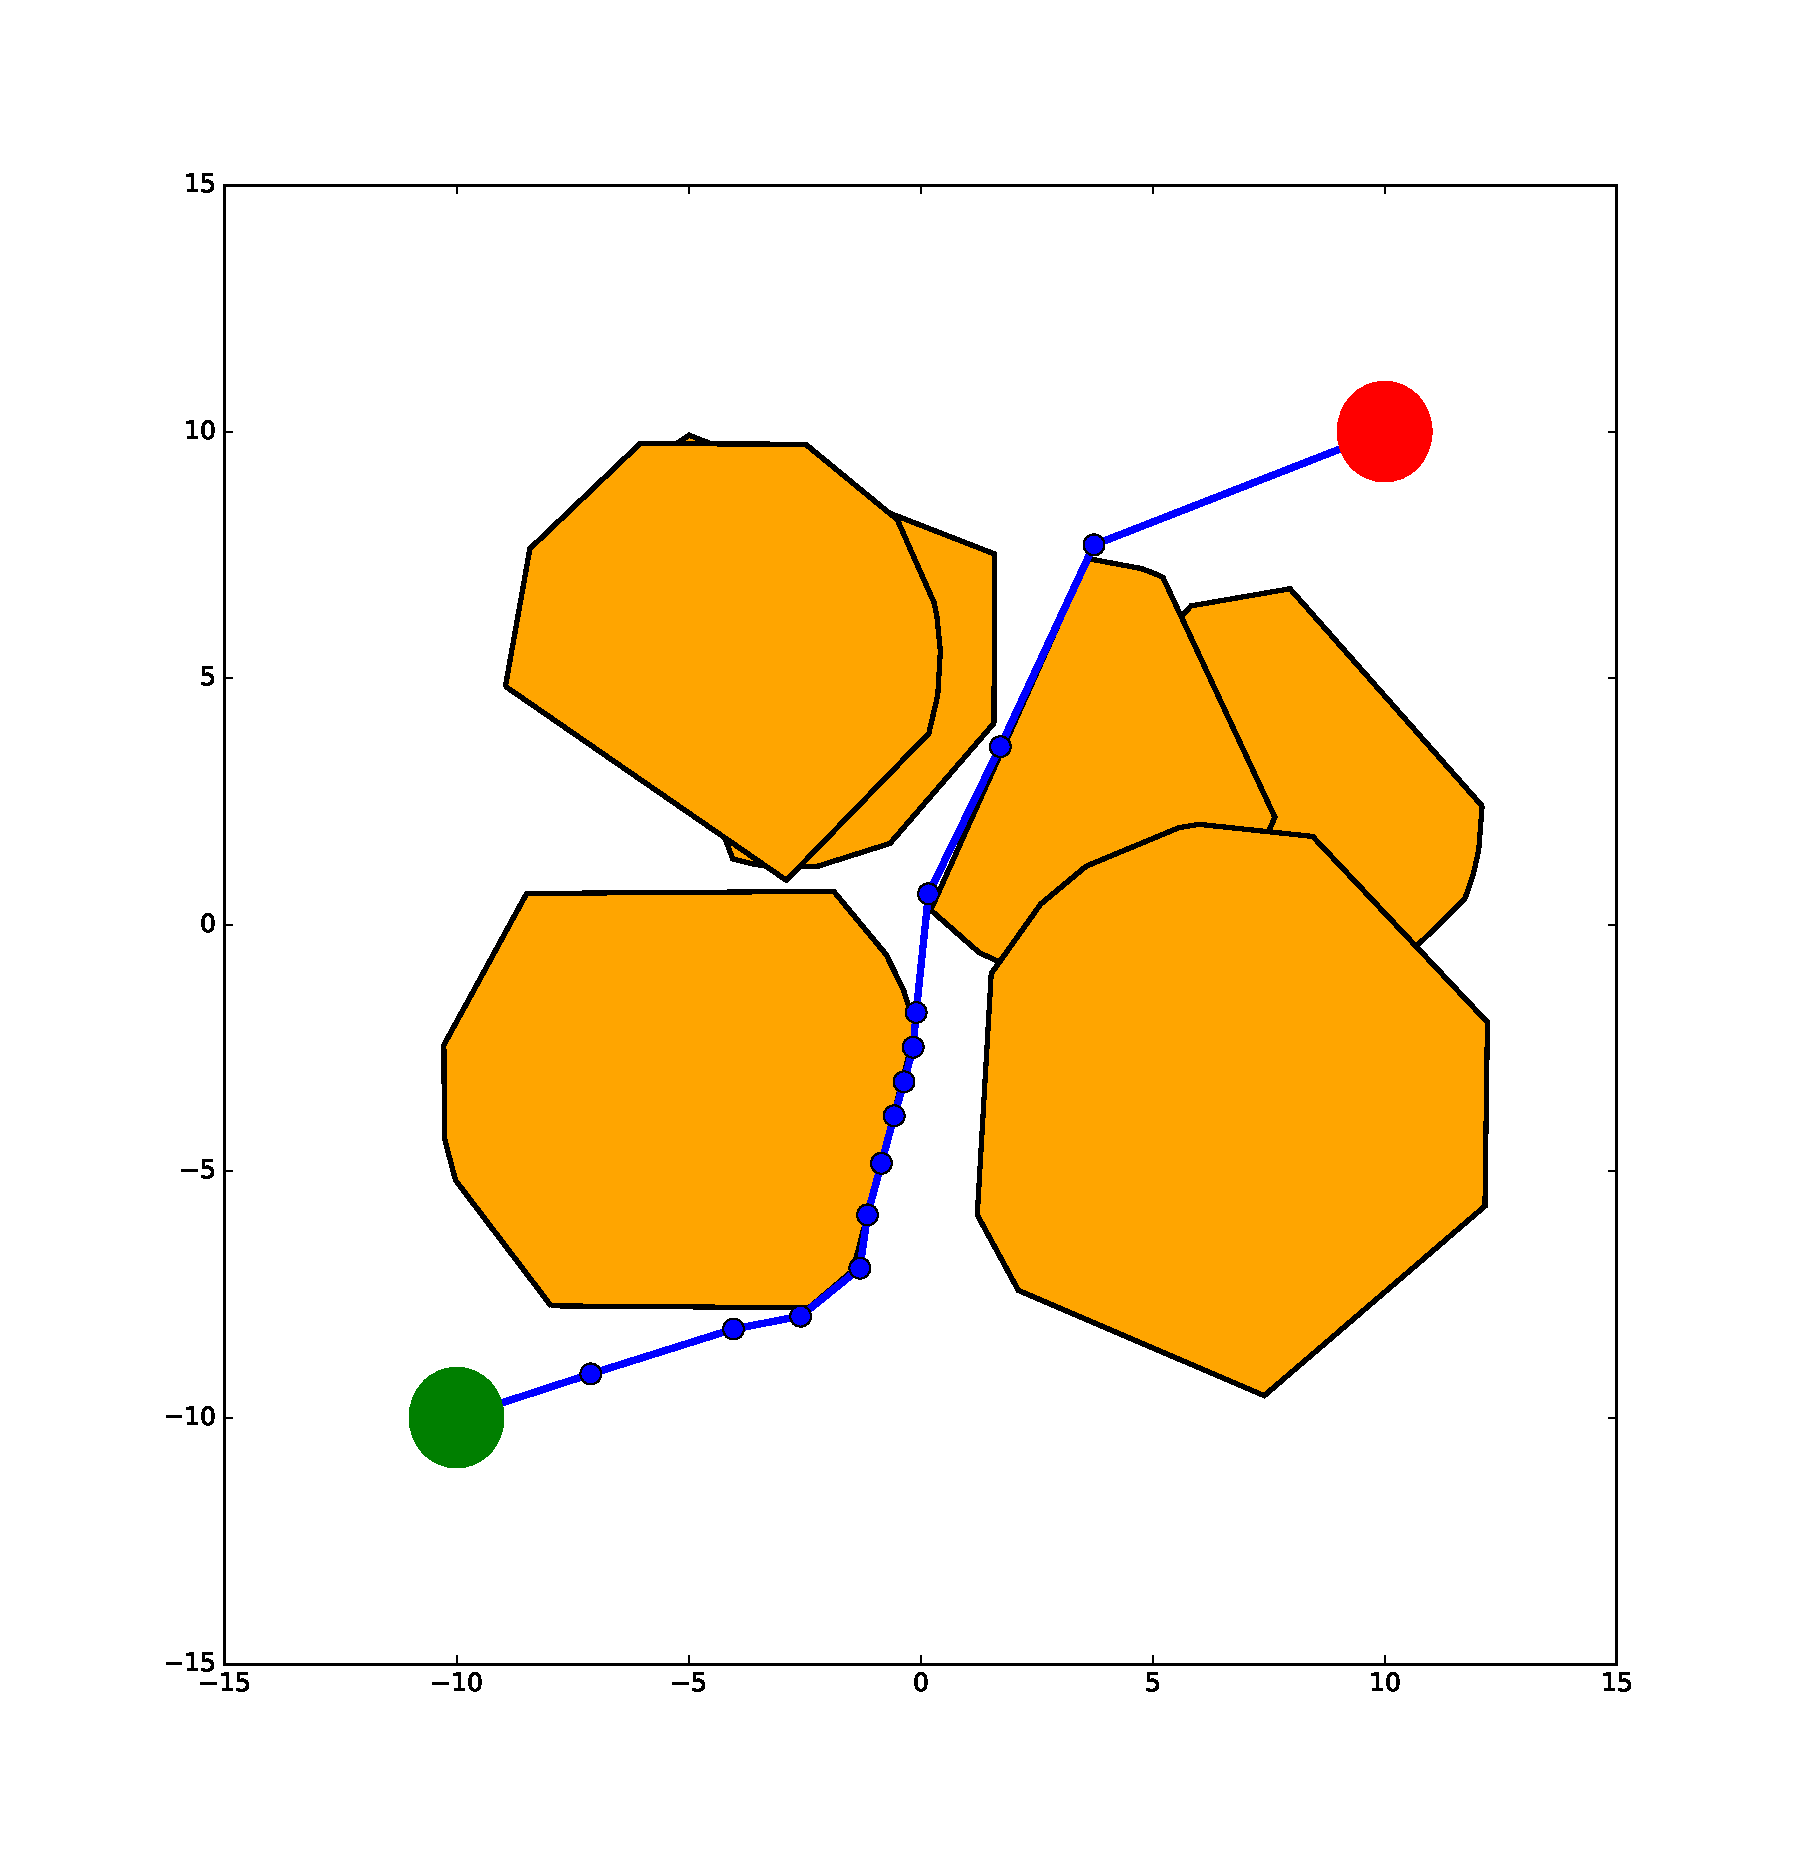
\includegraphics[width=0.32\textwidth]{2d_example_1.pdf}
    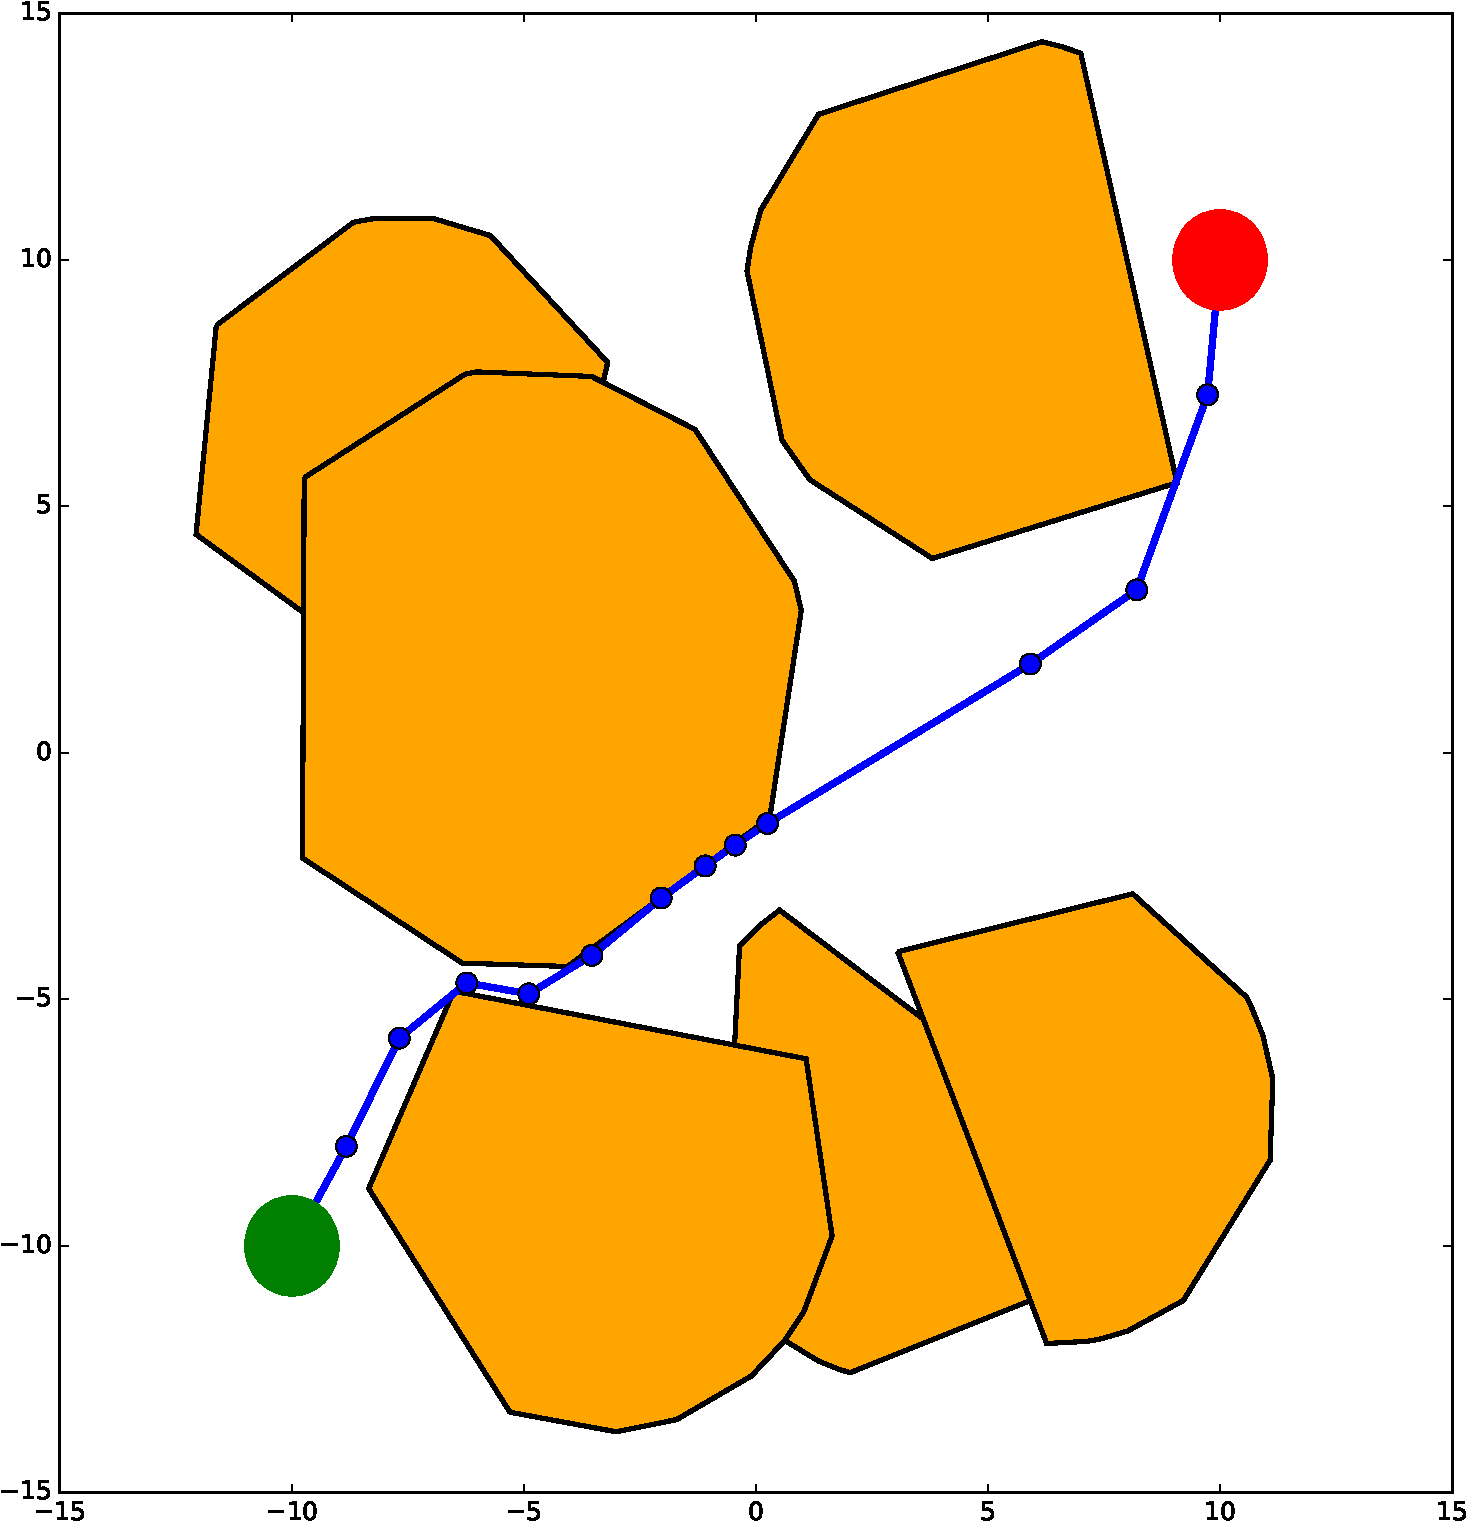
\includegraphics[width=0.32\textwidth]{2d_example_2.pdf}
    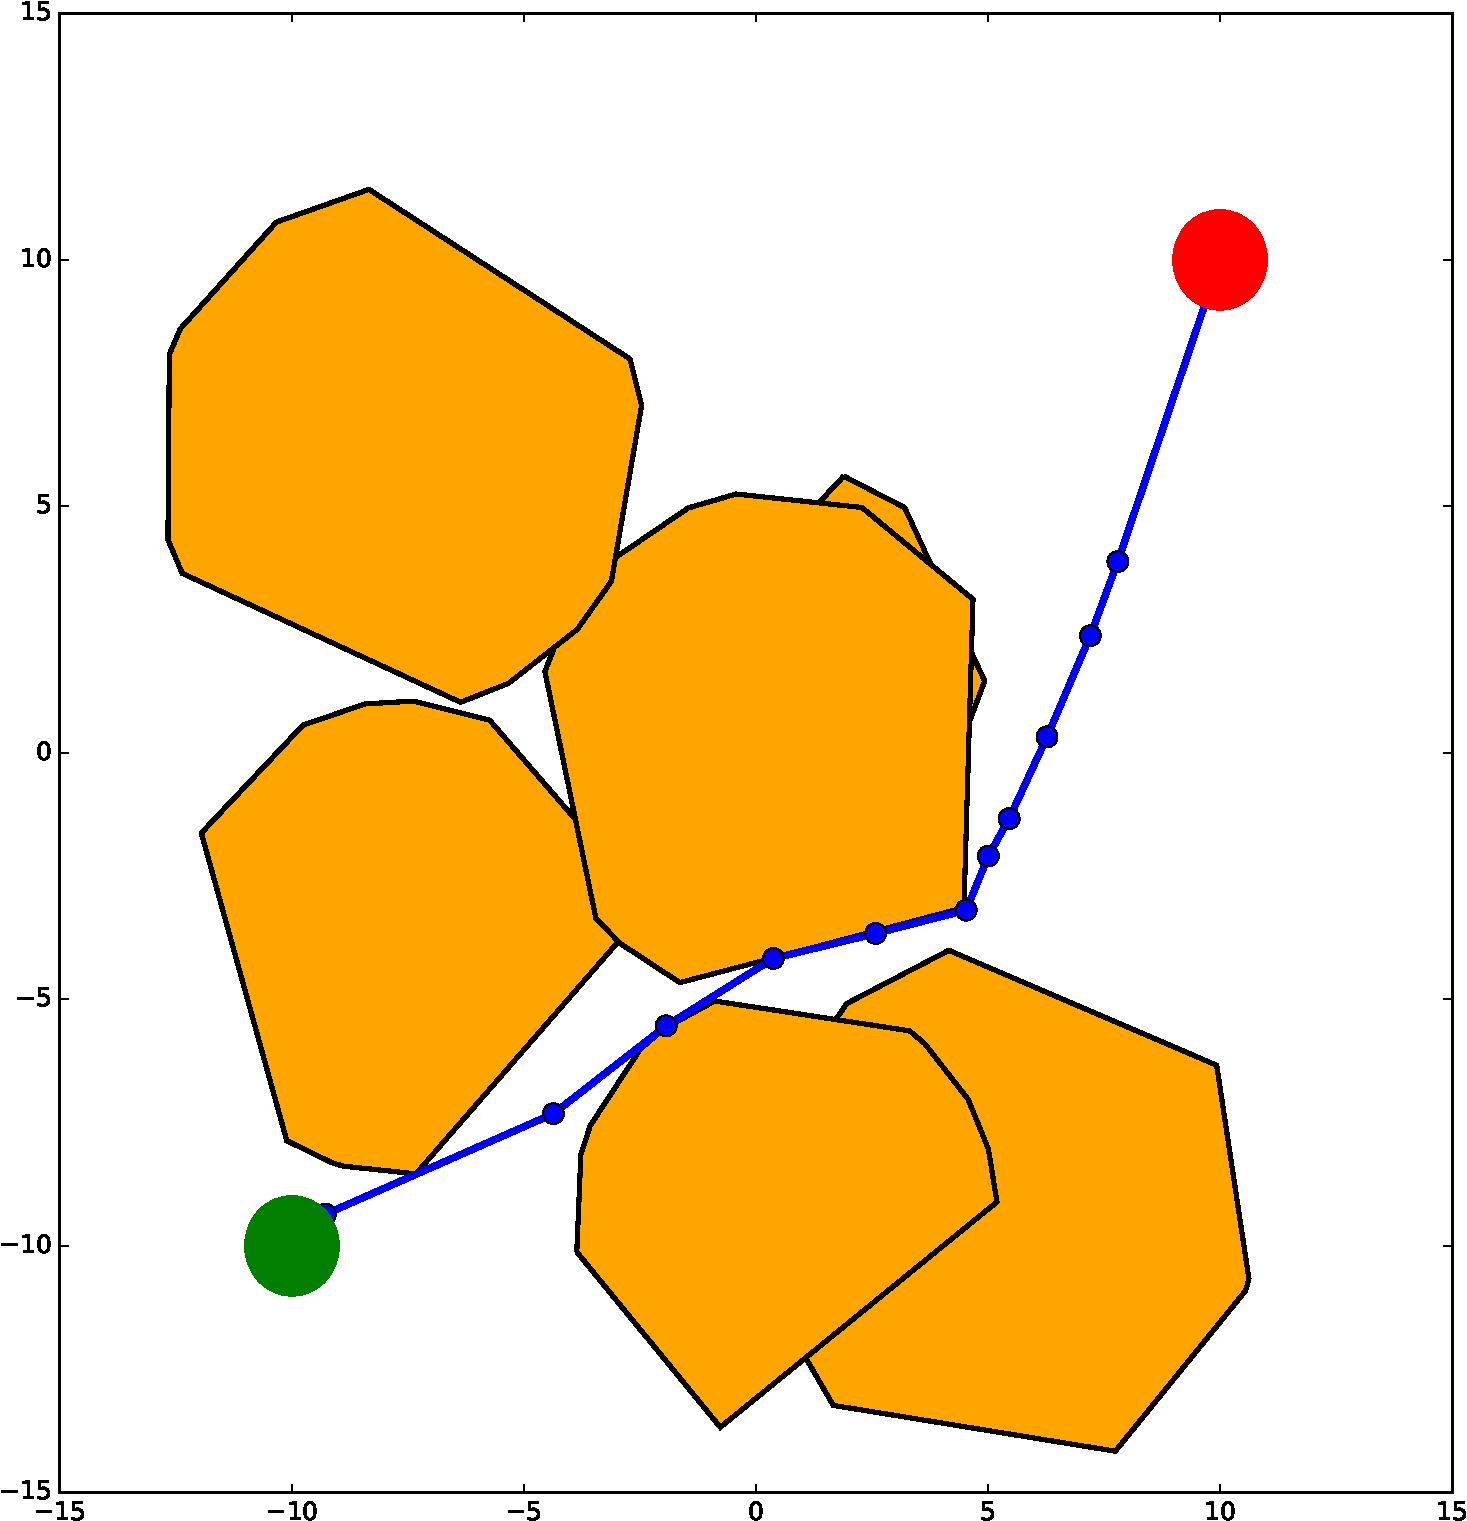
\includegraphics[width=0.32\textwidth]{2d_example_3.pdf} \\
    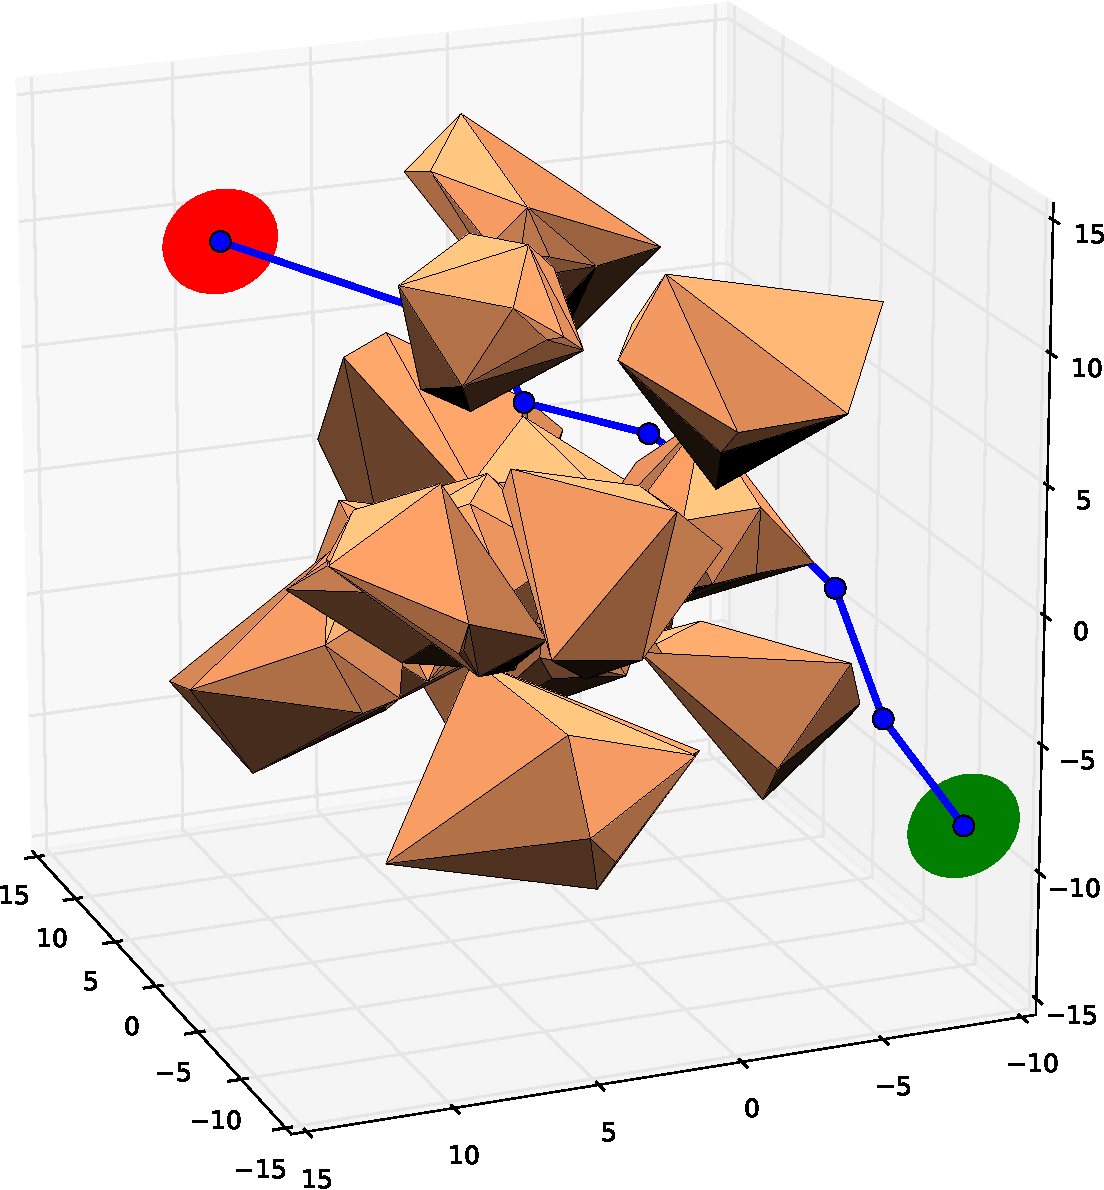
\includegraphics[width=0.32\textwidth]{3d_example_1.pdf}
    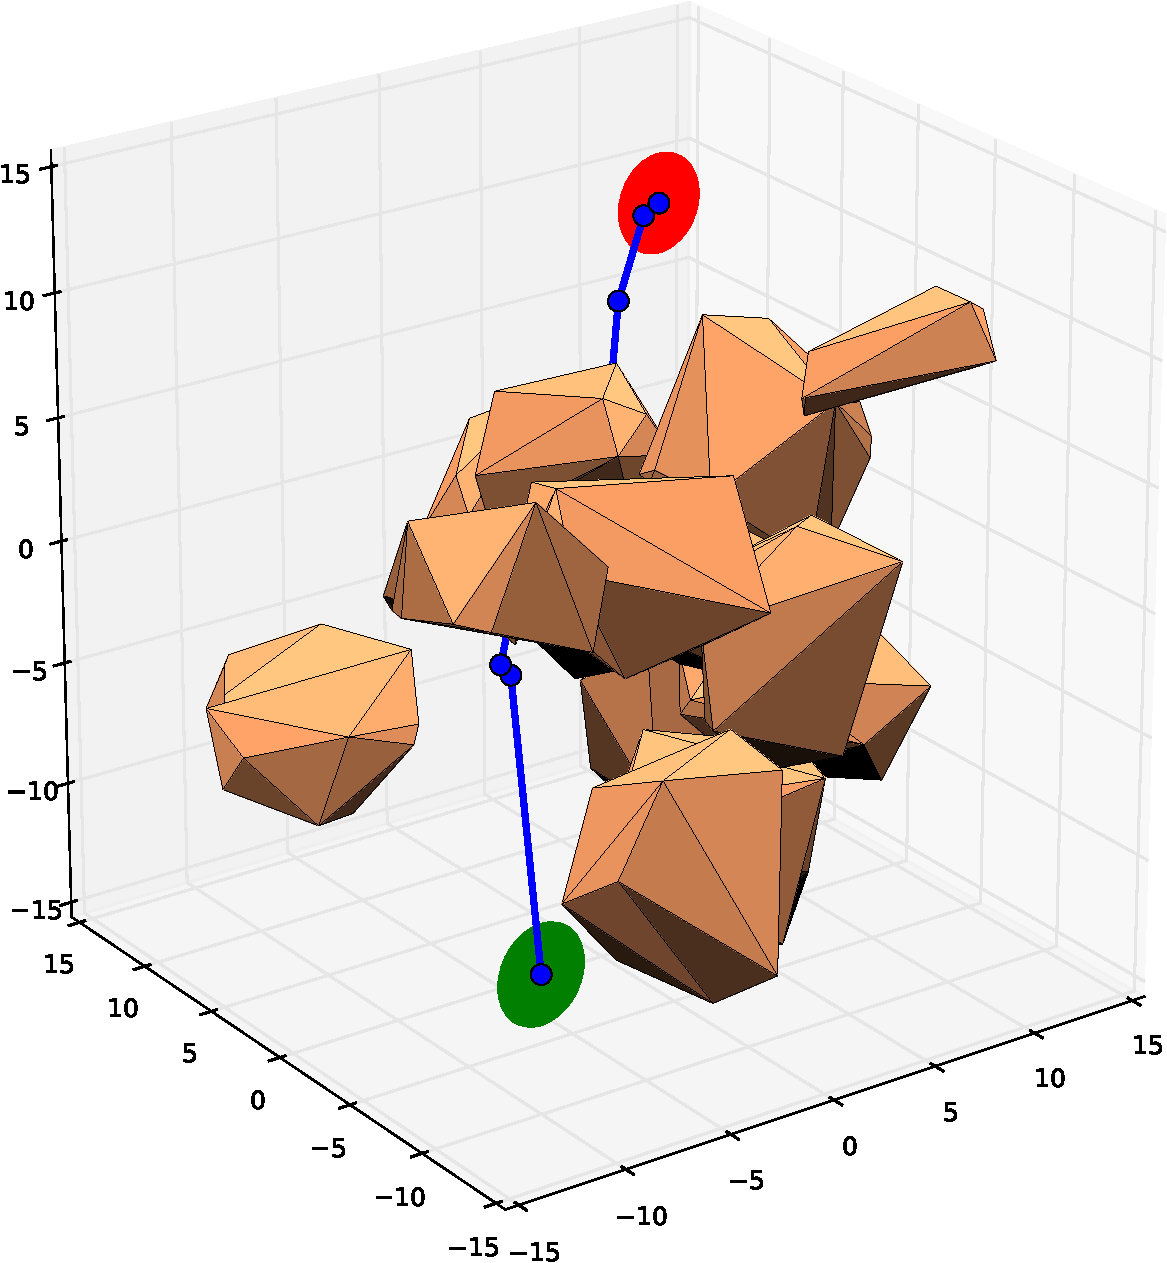
\includegraphics[width=0.32\textwidth]{3d_example_2.pdf}
    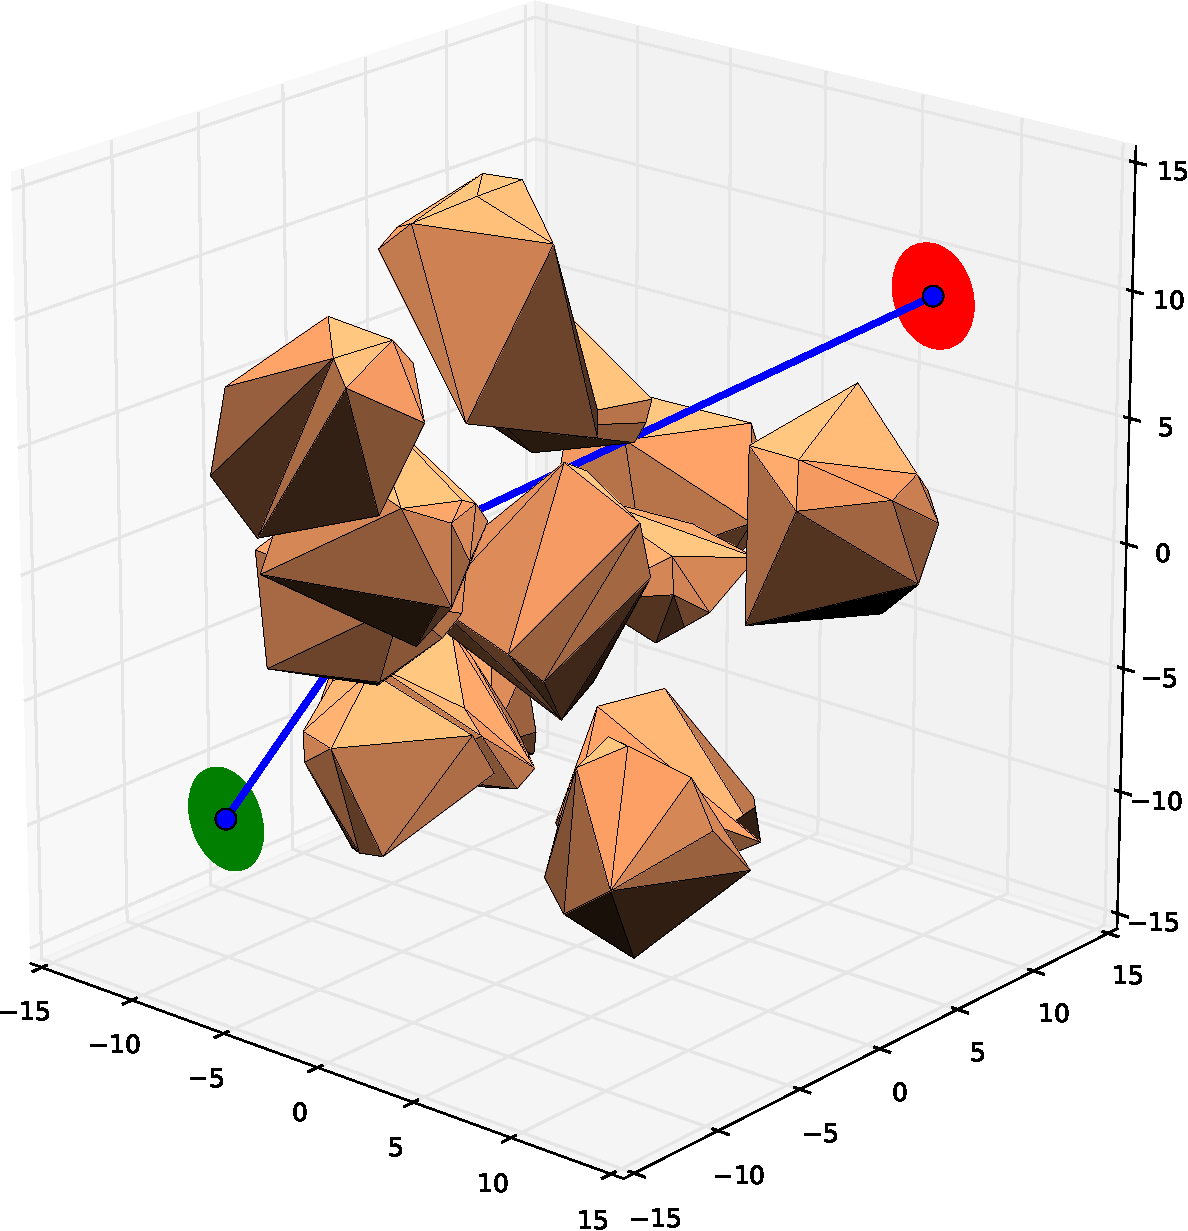
\includegraphics[width=0.32\textwidth]{3d_example_3.pdf}
    \caption{Examples of paths found in 2D and 3D scenes of random obstacles
    using the PRM algorithm. The green and red circles indicate the initial
    and goal configurations respectively. The blue path indicates the candidate
    solution through the space that connects the initial and goal
    configurations.}
    \label{fig:examples}
\end{figure}

\begin{figure}[h!]
    \centering
    \makebox[\textwidth][c]{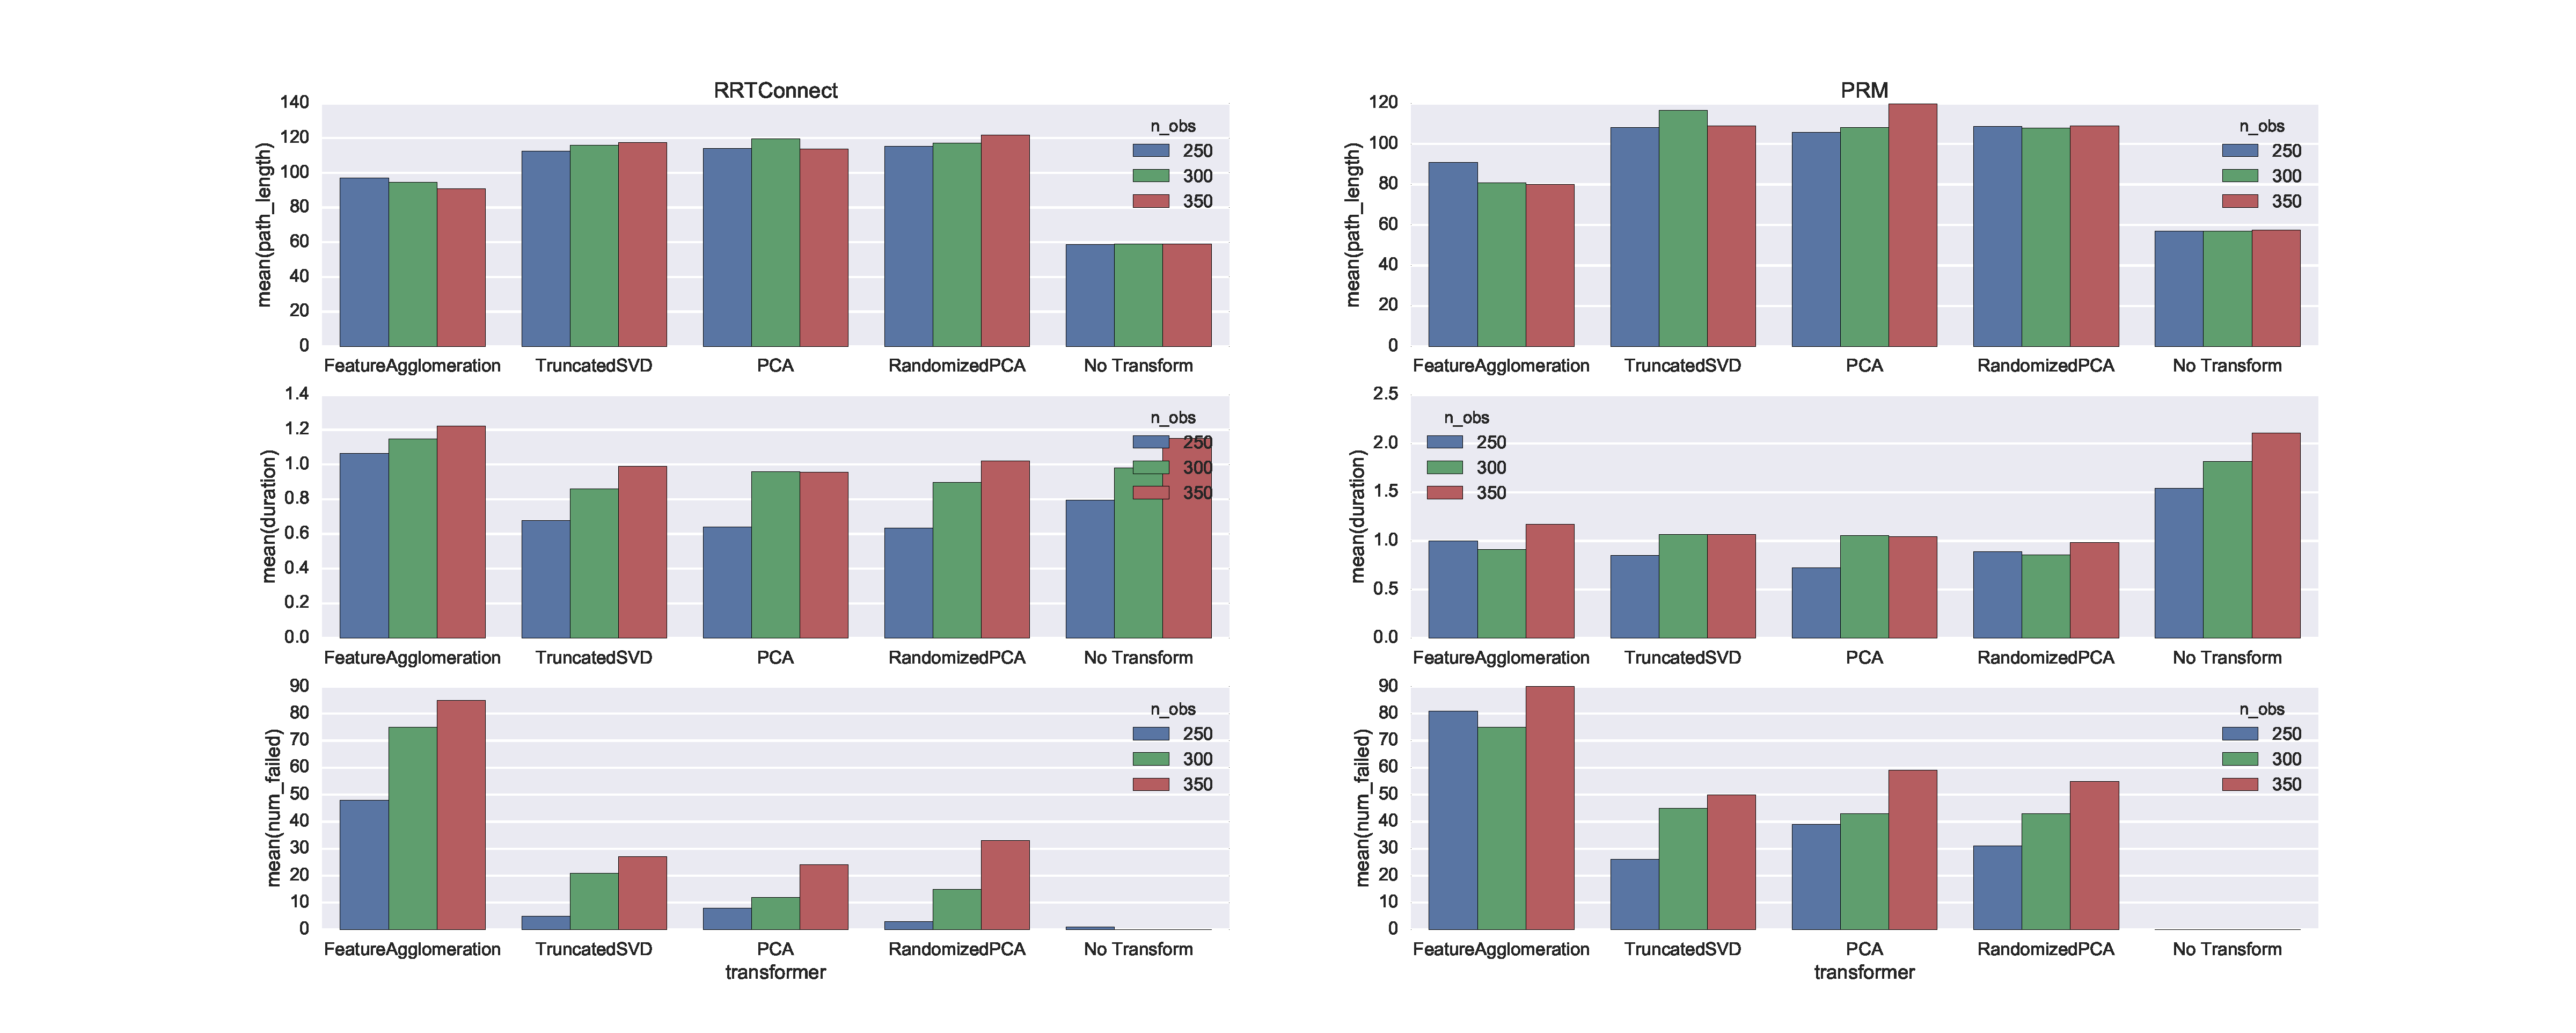
\includegraphics[width=1.5\textwidth]{plots}}
    \caption{Figure}
\end{figure}

You can see examples of our code running in Fig.~\ref{fig:examples}. The
results are listed in Figure WHAT. They show that 

\begin{algorithm}[ht] 
    \caption{$\Function{PRM}$~\cite{karaman2011sampling}}
    \label{alg:PRM}
    \begin{algorithmic}[1]
        \setcounter{ALC@line}{0}
        \vspace*{1mm}

        \STATE $V \leftarrow \{x_{\Var{init}}\} \cup \{\Var{SampleFree}_i\}_{i=1,\ldots,n}$
        \STATE $E \leftarrow \emptyset$
        \FORALL{$v \in V$}
            \STATE $U \leftarrow \Function{NearestNeighbors}(v)$
            \FORALL{$u \in U $}
                \IF{$\Function{CollisionFree}(v, u)$}
                    \STATE $E \leftarrow E \cup \{(v, u), (u, v)\}$
                \ENDIF
            \ENDFOR
        \ENDFOR
        \RETURN $G = (V, E)$

    \end{algorithmic}
\end{algorithm}


\begin{algorithm}[ht] 
    \caption{$\Function{Extend\_RRT($\mathcal{T}$,$q$)}$~\cite{kuffner2000rrt}}
    \label{alg:extend_RRT}
    \begin{algorithmic}[1]
        \setcounter{ALC@line}{0}
        \vspace*{1mm}
        \STATE $ q_{near} \leftarrow \Function{NEAREST\_NEIGHBOR($q$,$\;\mathcal{T}$)} $
        \IF{ $ \Function{NEW\_CONFIG($q$,$\;q_{near}$,$\;q_{new}$)} $}
            \STATE $ \mathcal{T}.\text{add\_vertex($q_{new}$)}; $
            \STATE $ \mathcal{T}.\text{add\_edge($q_{near}$,$\;q_{new}$)}; $
            \IF{$ q_{new} = q $}
                \RETURN $Reached$;
            \ELSE
                \RETURN $Advanced$;
            \ENDIF
        \ENDIF
        \RETURN $Trapped$;
    \end{algorithmic}
\end{algorithm}

\begin{algorithm}[ht] 
    \caption{$\Function{Connect\_RRT($\mathcal{T}$,$q$)}$~\cite{kuffner2000rrt}}
    \label{alg:connect_RRT}
    \begin{algorithmic}[1]
        \setcounter{ALC@line}{0}
        \vspace*{1mm}
        \REPEAT 
            \STATE $S \leftarrow \Function{EXTEND\_RRT($\mathcal{T}$,$\;q$)};$ 
        \UNTIL {$ \textbf{not} \; (S = Advanced)$}
        \RETURN $S;$
    \end{algorithmic}
\end{algorithm}

\begin{algorithm}[ht] 
    \caption{$\Function{RRTConnect($q_{init}$,$\;q_{goal}$)}$~\cite{kuffner2000rrt}}
    \label{alg:RRTConnect}
    \begin{algorithmic}[1]
        \setcounter{ALC@line}{0}
        \vspace*{1mm}
        \STATE $\mathcal{T}_a$.init($q_{init}$); $ \mathcal{T}_b$.init($q_{goal}$);
        \FOR{$k = 1 \ \TO \ K$}
            \STATE $q_{rand} \leftarrow \Function{RANDOM\_CONFIG()}$;
            \IF {$\textbf{not} \ (\Function{EXTEND\_RRT($\mathcal{T}_a$,$\;q_{rand} = Trapped$)})$}
                \IF {$ (\Function{CONNECT\_RRT($\mathcal{T}_b,q_{new}$}) = Reached $}
                    \RETURN $ \Function{PATH($\mathcal{T}_a,\mathcal{T}_b$)} $
                \ENDIF
            \STATE \Function{SWAP($\mathcal{T}_a,\mathcal{T}_b)$}
            \ENDIF
        \ENDFOR
        \RETURN $Failure$
    \end{algorithmic}
\end{algorithm}

% \begin{algorithm}[ht] 
%     \caption{$\Function{RRT}^*$~\cite{karaman2011sampling}}
%     \label{alg:RRTConnect}
%     \begin{algorithmic}[1]
%         \setcounter{ALC@line}{0}
%         \vspace*{1mm}

%         \STATE $V \leftarrow \{x_{\Var{init}}\}$
%         \STATE $E \leftarrow \emptyset$
%         \FOR{$i = 1 \ \TO \ n$}
%             \STATE $\xr \leftarrow \Var{SampleFree}_i$
%             \STATE $\xnearest \leftarrow \Function{Nearest}(G = (V, E), \xr)$
%             \STATE $\xnew \leftarrow \Function{Steer}(\xnearest, \xr)$
%             \IF{$\Function{ObstacleFree}(\xnearest, \xnew)$}
%                 \STATE $\xnear \leftarrow \Function{Near}(G = (V, E), \xnew,
%                 \min \{\gamma \cdot \Function{RRT}(\log(|V|) / |V|)^{1 / d}, \eta\})$
%                 \STATE $V \leftarrow V \cup \{\xnew\}$
%                 \STATE $\xmin \leftarrow \xnearest$
%                 \STATE $\cmin \leftarrow \Function{Cost}(\xnear) +
%                 c(\Function{Line}(\xnearest, \xnew))$
%                 \FORALL{$\xnear \in X_{\Var{near}}$}
%                     \STATE $C \leftarrow \cost(\xnear) + \linef{\xnear, \xnew}$
%                     \IF{$\Function{CollisionFree}(\xnear, \xnew) \wedge C < \cmin$}
%                         \STATE $\xmin \leftarrow \xnear$
%                         \STATE $\cmin \leftarrow C$
%                     \ENDIF
%                     \STATE $E \leftarrow E \cup \{(\xmin, \xnew)\}$
%                 \ENDFOR
%                 \FORALL{$\xnear \in X_{\Var{near}}$}
%                     \STATE $C \leftarrow \cost(\xnew) + \linef{\xnew, \xnear}$
%                     \IF{$\Function{CollisionFree}(\xnew, \xnear) \wedge C < \cost(\xnear)$}
%                         \STATE $\xparent \leftarrow \Function{Parent}(\xnear)$
%                         \STATE $E \leftarrow (E \backslash \{(\xparent, \xnear)\}) \cup \{(\xnew, \xnear)\}$
%                     \ENDIF
%                 \ENDFOR
%             \ENDIF
%         \ENDFOR
%         \RETURN $G = (V, E)$

%     \end{algorithmic}
% \end{algorithm}

\begin{algorithm}[ht] 
    \caption{$\Function{Dimensionality Reduction}$}
    \label{alg:DR}
    \begin{algorithmic}[1]
        \setcounter{ALC@line}{0}
        \vspace*{1mm}

        \STATE Specify dimension, dimensionality reduction technique, and obstacle information
        \STATE Generate random obstacles based off of obstacle information
        \STATE Fit dimensionality reduction transform to the space
        \STATE Transform the space
        \STATE Run PRM* or RRTConnect over the space
        \STATE Inverse transform the path back to the original dimension
        \STATE Check for collisions
        \RETURN Path\_length, duration, num\_failed
    \end{algorithmic}
\end{algorithm}


\bibliographystyle{plain}
\bibliography{bib}

\end{document}
